\documentclass{scrbook}
\usepackage{graphicx} % Required for inserting images
\usepackage{tabularx} % Required for fixed width tables
\usepackage{scrlayer-scrpage} % Required for the subtitles
\usepackage{url} % Required for the URLs
\usepackage{hyperref} % Required for the URLs
\usepackage{listings} % Required for the code snippets

% Put the caption of the snippets at the bottom
\lstset{
    captionpos=b
}


\title{WWW and W3C}
\subtitle{Ambient intelligence course (A.Y. 2025/2026)\\Topic taught by Prof. Michele Ruta}
\author{Gabriele Colapinto}
\date{\today}

\begin{document}

\maketitle
\thispagestyle{empty}

{\Large\textbf{License}} \\
{Notes from Ambient intelligence (A.Y. 2025/2026) by Gabriele Colapinto. 
Course taught by professors Michele Ruta, Floriano Scioscia, Arnaldo Tomasino, Davide Loconte — 
Licensed under CC BY-NC 4.0.\\
\url{https://creativecommons.org/licenses/by-nc/4.0/}}

\vspace*{\fill}
\rule{\textwidth}{0.2pt}
\small{© 2025 Gabriele Colapinto \\
Released under the \href{https://creativecommons.org/licenses/by-nc/4.0/}{Creative Commons Attribution–NonCommercial 4.0 International License}}

\clearpage

\tableofcontents

\chapter{Defining the World Wide Web}

The World Wide Web is one of the most transformative information systems ever created, fundamentally reshaping how we access, share, and interact with knowledge. Understanding its core definitions is not merely an academic exercise; it is a strategic necessity for anyone involved in building or utilizing digital technologies. The Web's architecture is built upon a set of elegant and powerful principles, and grasping these foundational ideas is the first step toward appreciating its design and impact. \\

In technical and academic literature, the World Wide Web is commonly referred to by the acronyms \textbf{WWW} or \textbf{W3}. While these terms are used interchangeably, they point to two distinct but complementary definitions that capture both the philosophical ambition and the technical function of the system.

\section{Core Definitions}

The source materials present two primary definitions that together encapsulate the essence of the Web: \\

"The universe of network-accessible information, the embodiment of human knowledge." \\

This first definition speaks to the Web's ultimate goal and philosophical scope. It positions the WWW not just as a technology, but as a global repository for human knowledge, a vast, interconnected library accessible to all. \\

"A wide-area hypermedia information retrieval initiative aiming to give universal access to a large universe of documents." \\

The second definition is more technical and functional. It highlights the key mechanisms and objectives: it is a \textit{wide-area} system (global), based on \textit{hypermedia} (linked multimedia), designed for \textit{information retrieval} (finding documents), with the central aim of providing \textit{universal access}. \\

These definitions provide a framework for understanding the Web's purpose. To fully appreciate its architecture, however, we must first examine its historical origins.

\chapter{A Brief History of the Web's Genesis}

The World Wide Web did not emerge from a corporate boardroom but from a scientific community grappling with a significant challenge: information management. In the late 1980s, researchers at CERN, the European Organization for Nuclear Research, faced the difficult task of sharing vast and diverse sets of documents across a heterogeneous collection of computers and networks. The Web was born as a practical solution to this problem, conceived as a distributed information system to streamline access to knowledge within the laboratory. \\

The development of the Web can be traced through several key milestones: \\

\begin{itemize}
    \item
    \textbf{March 1989:} Tim Berners-Lee, a scientist at CERN, authored a proposal for a distributed information system. This document laid out the conceptual groundwork for what would become the World Wide Web, aiming to solve the challenge of information loss and difficult collaboration among researchers.

    \item
    \textbf{December 1990:} Berners-Lee brought his proposal to life. He defined the Web’s foundational concepts, developed the world's first web browser and server software, and launched the first website. This inaugural site was hosted on his NeXT computer and was dedicated to the WWW project itself, available at the address: \\ \texttt{http://info.cern.ch/hypertext/WWW/TheProject.html}.

    \item
    \textbf{January 1991:} The early WWW system, comprising the simple browser server software and a supporting library, was released internally to the high-energy-physics community via the CERN program library. This marked the first practical deployment of the Web within a specific user group.

    \item
    \textbf{April 1993:} In a pivotal move that catalyzed the Web's global expansion, CERN released the project's source code into the public domain. This decision removed all barriers to adoption, allowing anyone to use, modify, and build upon the core technology freely.
\end{itemize}

\section{Rapid Growth and Adoption}

The public release of the Web's source code triggered an immediate and explosive period of growth. By late 1993, just months after its public debut, there were over 500 known web servers, and the Web already accounted for 1\% of all internet traffic. The momentum continued to build exponentially. By the end of 1994, the Web had grown to an astonishing 10,000 servers and 10 million users. Significantly, 2,000 of these 10,000 servers (20\%) were commercial, signaling that the Web was rapidly transitioning from a research project into a powerful platform for global commerce and communication. \\

This remarkable adoption was not accidental. It was the direct result of the elegant and powerful foundational concepts that underpinned the Web's architecture from its very inception.

\chapter{Foundational Concepts of the Web Architecture}

The success of the World Wide Web is rooted in a few revolutionary concepts that directly addressed the critical problems of information access that existed before its creation. These principles were designed to create a system that was simple, decentralized, and universally accessible, forming the pillars of the Web's architecture.

\section{Universal Readership}

Before the WWW, accessing information from different computers was a complex and frustrating task. A user often needed different terminals and specialized client programs to connect to each machine. This created a fragmented and non-interoperable information landscape where accessing a document on one system required entirely different software and procedures than accessing a document on another. The result was a system that was costly, difficult to use, and a significant barrier to the free exchange of information. \\

The principle of \textbf{Universal Readership} was Tim Berners-Lee's proposed solution and the foundational objective of the Web. It is the simple yet radical idea that any information should be accessible from any type of computer, in any country. Furthermore, an authorized person should only need a single, simple program—a browser—to access this universe of information. This concept eliminated the need for specialized clients for each server, creating a unified and interoperable information space.

\section{Hypertext and Hypermedia}

At the core of the Web's document structure is the concept of hypertext. \\

\textbf{Hypertext} is defined simply as "text with links." While the idea was not new—books have long used references, footnotes, and tables of contents to link different parts of a text—its implementation in a global, networked system was transformative. Hypertext represented a fundamental paradigm shift in how information is consumed. It allows the reader to escape the rigid, sequential organization imposed by the author of a traditional document. By following links, the user personalizes the "fruition" of the content, creating their own path through the information. For the first time on a mass scale, control over the navigation of knowledge was transferred from the writer to the reader. \\

\textbf{Hypermedia} is the natural evolution of hypertext. It extends the concept of linking beyond simple text to integrate other media forms, such as graphics, movies, and sound, directly into a single document. This innovation transformed web documents from plain text files into rich, complex compositions. As a result, the term "document" became insufficient to describe these composite entities, leading to the adoption of the more general and accurate term \textbf{"resource"}. \\

To connect these new hypermedia resources across a global network, a standardized and unambiguous addressing system was essential. This need gave rise to the Uniform Resource Locator.

\chapter{The Uniform Resource Locator (URL): The Web's Addressing System}

The Uniform Resource Locator (URL) is the critical addressing protocol that makes the Web possible. It provides a standardized, unambiguous method for locating any resource on the internet, regardless of where it is or what protocol is used to access it. Every link on the Web is powered by a URL, which acts as a unique, network-wide address for the target resource. \\

\section{The Anatomy of a URL}

\begin{figure}
    \centering
    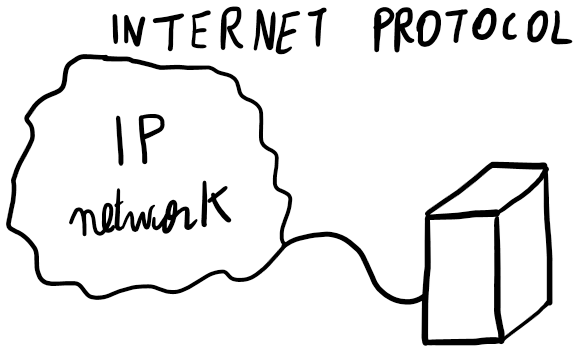
\includegraphics[width=0.5\linewidth]{Images/Internet_protocol.png}
    \caption{A server connected to an IP network to make its resources accessible to the Internet}
\end{figure}

A URL is deconstructed into two primary conceptual parts, which correspond to distinct layers of the ISO/OSI networking model and answer two fundamental questions: "Where is the resource?" and "How should I handle it?" \\

The first part is the \textbf{Resource Identifier}, which specifies the location of the resource (See figure 4.1). It is itself composed of two elements:

\begin{itemize}
    \item
    The \textbf{Network Address} is used to locate the specific machine (the server) on the global network. This function operates at Layers 3 and 4 of the ISO/OSI model, utilizing network protocols like TCP/IP.

    \item
    The \textbf{Folder} is used to pinpoint the specific resource \textit{within} that machine, providing the path to the file on the server's file system.
\end{itemize}

The second part is the \textbf{Access Protocol}, which specifies the application-level protocol the client must use to correctly process the resource once it has been retrieved. This function corresponds to Layer 7 of the ISO/OSI model and includes protocols such as HTTP (Hypertext Transfer Protocol), FTP (File Transfer Protocol), or SMTP (Simple Mail Transfer Protocol).

\section{Core Principle: Resolvability}

\begin{figure}
    \centering
    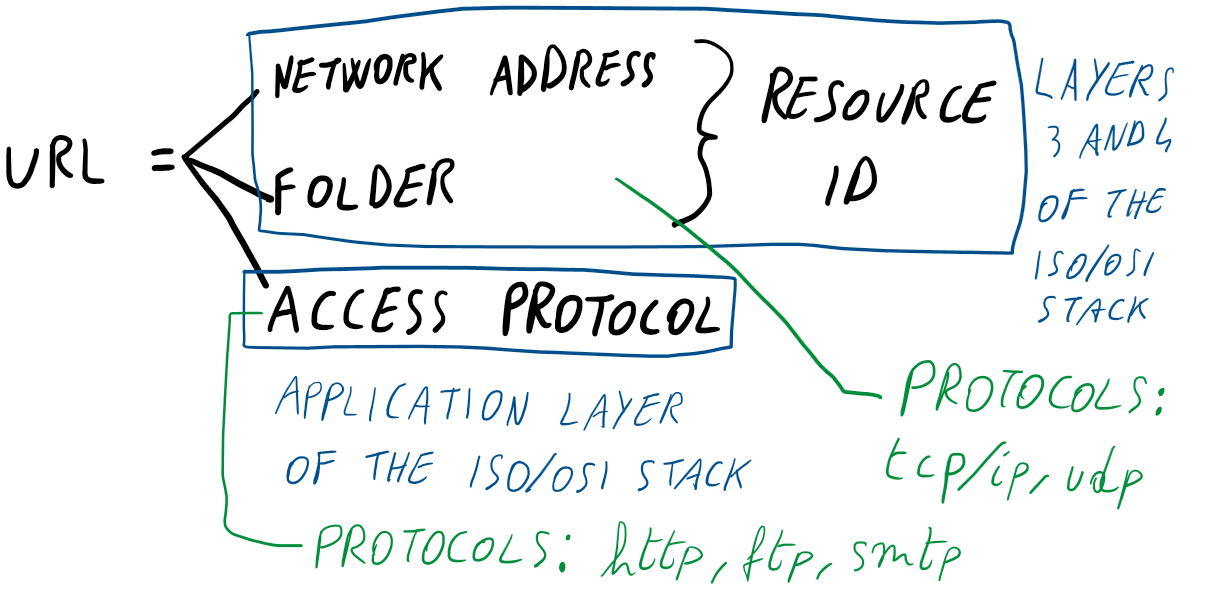
\includegraphics[width=0.7\linewidth]{Images/URL_resolvability.png}
    \caption{URL resolvability}
\end{figure}

A URL's primary function is defined by its \textbf{resolvability}. This is a core requirement of the architecture, formally defined as: \\

The capacity to start from the URL and derive its 3 constituent components (network address, folder, access protocol). \\

Resolvability is an \textbf{automatic process} executed by software (like a web browser). The sequence is as follows:

\begin{enumerate}
    \item
    The URL is parsed, or broken down, into its constituent parts.

    \item
    The network address is used to locate the host machine across the network. This typically involves a DNS (Domain Name Service) client to convert a symbolic name (e.g., \texttt{www.example.com}) into a machine-readable IP address.

    \item
    The folder path is then used to find the specific resource on the located machine.

    \item
    Once found, the resource is transferred back to the client that made the request.

    \item
    Finally, the access protocol from the URL dictates which client-side application or handler is activated to correctly manage, process, and present the resource to the user.
\end{enumerate}

\section{Essential Properties of a URL}

To function effectively as a global addressing system, URLs must adhere to several essential properties:

\begin{itemize}
    \item
    \textbf{Persistence:} A URL should maintain a stable, one-to-one correspondence with its associated resource over time. If the resource does not change, its URL should not change either. This ensures that links remain reliable.

    \item
    \textbf{Unambiguity and Uniqueness:} The correspondence between a URL and a resource must be unambiguous. A single resource must correspond to a single, unique URL, and that URL must point to only that resource. This prevents conflicts and ensures that users always reach the intended destination.

    \item
    \textbf{Readability and Information Hiding:} This property is a sophisticated dual requirement that reflects core computer science principles of its era. A URL must be readable by both humans and machines. However, it must also adhere to the principle of \textit{information hiding}, a concept that gained prominence with Object-Oriented Programming (OOP). In OOP, this principle was used to manage complexity and protect a programmer's intellectual property by separating a public interface from its private implementation. The URL's design consciously adopts this paradigm: the symbolic, human-readable domain name is the "public interface," while the underlying, machine-specific IP address is the "private implementation detail." This hidden information is not secret, but it can only be retrieved by processing the URL with an appropriate application, such as a DNS client.

    \item
    \textbf{Extensibility:} The URL framework was ingeniously designed to be extensible. It was built not only to cover existing access schemes of its time (like FTP) but also to accommodate future, yet-to-be-invented protocols. A new protocol can be added to the list of possible access schemes without requiring any changes to the fundamental URL architecture or the existing business and infrastructure built upon it.
\end{itemize}

\chapter{The Foundational Client-Server Architecture of the Web}

\begin{figure}
    \centering
    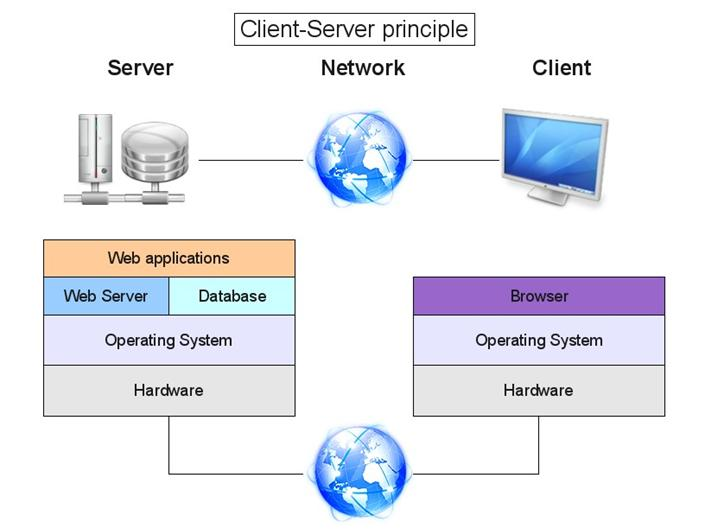
\includegraphics[width=\linewidth]{Images/Client_server_principle.jpg}
    \caption{WWW client-server architecture}
\end{figure}

At its core, the Web operates on a client-server principle, a model that defines the roles and interactions of the two primary components involved in any web-based communication.

\begin{table}[h!]
    \centering
    \begin{tabularx}{\textwidth}{|X|X|} \hline
        \textbf{Client} & \textbf{Server}
        \\ \hline

        Acts as the \textbf{requester} in the communication exchange. &
        Manages and responds to a large number of requests from multiple clients.
        \\ \hline

        Composed of a browser (the application layer) running on an operating system. &
        Composed of a web server application, an operating system, and often a database to manage information.
        \\ \hline

        Typically utilizes \textbf{lightweight hardware}, as it generally manages only a small number of requests at a time. &
        Requires powerful hardware and high-performance network interfaces to handle multitasking and process numerous concurrent requests, often managed through multi-threaded server applications.
        \\ \hline
    \end{tabularx}
    \caption{Comparison of client and server}
\end{table}

The communication process follows a request-reply sequence. A user action on the client-side generates a request, which is sent across the World Wide Web network, often using a socket association for communication. This request travels through the network until it reaches the target server machine. On the server, a web server application, often referred to as a "demon," is perpetually listening on a specific port for incoming traffic (e.g., for the HTTP protocol). This application pre-processes the request, directs it to the appropriate web application for processing, and formulates a reply. The reply is then sent back through the network to the client, where the browser visualizes the result for the user. \\

This client-server model is not unique to web browsing; it is the foundational principle for nearly all web-based applications, including the File Transfer Protocol (FTP), email systems, and the Domain Name System (DNS). This explosive growth in a decentralized system created an urgent need for a coordinating body capable of stewarding its technical architecture, a role the W3C was explicitly designed to fill.

\chapter{The World Wide Web Consortium (W3C): Genesis and Guiding Principles}

The World Wide Web Consortium (W3C) is the primary international community established to develop open standards that ensure the long-term growth, stability, and interoperability of the Web (See figure 6.1). Founded in 1994, it was created to coordinate the evolution of web technologies and protocols in a structured, consensus-driven manner.

\begin{itemize}
    \item
    \textbf{Founder:} Tim Berners-Lee

    \item
    \textbf{Year Founded:} 1994

    \item
    \textbf{Coordinating Hosts:} MIT (United States), ERCIM (Europe), and Keio University (Japan)

    \item
    \textbf{Scale:} The consortium includes more than 350 members, over 100 distinct groups, and maintains 92 offices worldwide to manage its global initiatives.
\end{itemize}

\begin{figure}
    \centering
    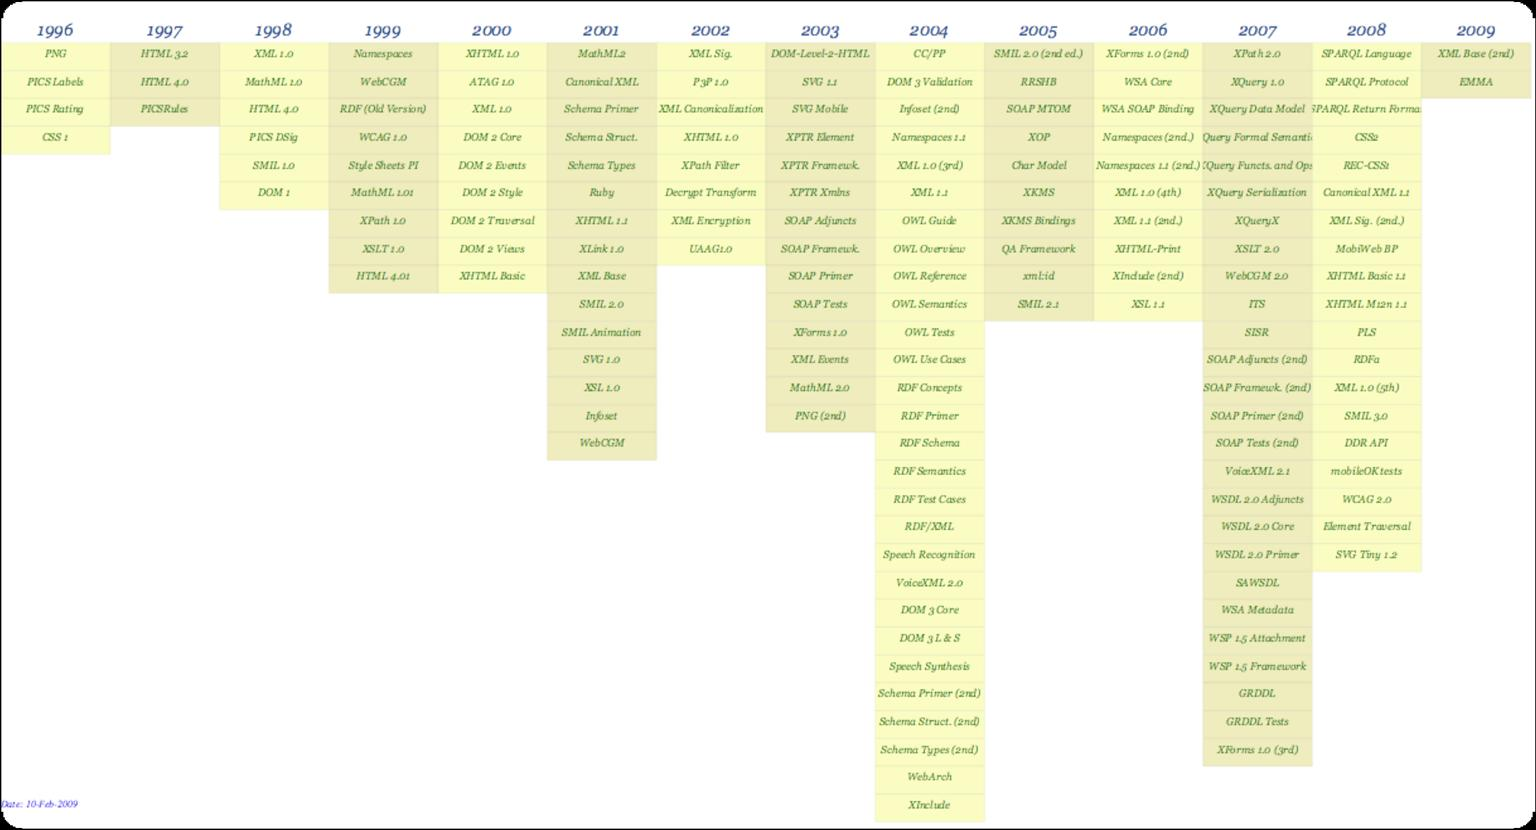
\includegraphics[width=\linewidth]{Images/W3C_standards.jpg}
    \caption{W3C standards}
\end{figure}

\section{The Four Core Goals of the W3C}

The mission of the W3C is guided by four fundamental purposes that shape its strategic direction and technical work. \\

\begin{itemize}
    \item
    \textbf{Web for Everyone:} This goal represents the mission to enable universal human communication, commerce, and knowledge sharing. The W3C promotes principles and technologies that ensure the Web is accessible to all people, without limits based on race, sex, or cultural background, extending to communication between humans, humans and machines, and machine-to-machine interactions.

    \item
    \textbf{Web for Everything:} Flowing from the first principle, this goal asserts that Web access should be available from any device, irrespective of its hardware or software constraints (See figure 6.2). The W3C advocates for standards that prevent the fragmentation of the Web into device-specific silos, thereby promoting democratic access to information and services for all users, regardless of their technical capabilities.

    \item
    \textbf{Knowledge Base:} The W3C is responsible for creating, devising, and maintaining a comprehensive repository of problems and their corresponding solutions. This knowledge base serves as a crucial resource to support diverse user communities around the world, enabling them to resolve complex technical issues related to Web exploitation and access.

    \item
    \textbf{Trust and Confidence:} Established in the early days of the Web when public trust in the new medium was low, this goal focuses on promoting technologies that support secure transactions and trusted collaboration. This has been critical for the growth of essential web functions such as e-commerce, online banking, and cross-border agency interactions, where confidence in the underlying tool is paramount for all involved actors.
\end{itemize}

To execute this ambitious mission, the W3C relies on a well-defined organizational structure designed to foster collaboration and build global consensus.

\begin{figure}
    \centering
    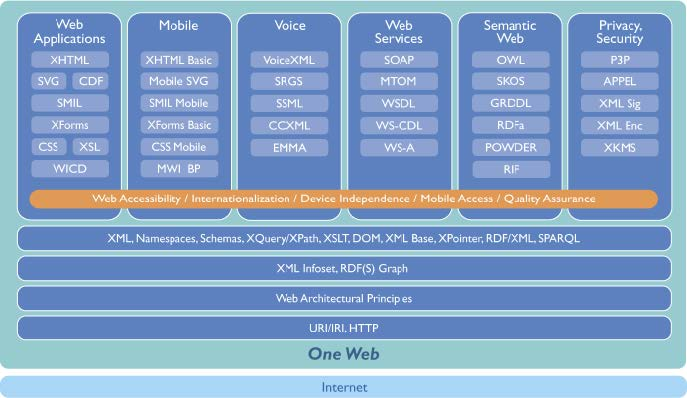
\includegraphics[width=\linewidth]{Images/W3C_technology_stack.jpg}
    \caption{W3C technology stack for different applications}
\end{figure}

\chapter{The Organizational Structure of the W3C}

A well-defined, multi-stakeholder organizational structure is critical for managing the technical and strategic evolution of the Web. The W3C's framework is designed to balance the interests of its diverse membership while maintaining a clear process for technical development and governance.

\section{Membership and Representation}

\begin{itemize}
    \item
    \textbf{Members:} Membership in the W3C is open to all entities, including corporations, non-profits, and academic institutions. While the consortium does not have a membership class specifically tailored for individuals, an individual may join as an Affiliate Member.

    \item 
    \textbf{Advisory Committee (AC):} Each member organization must appoint a representative to the Advisory Committee. The AC is a critical body that represents the collective interests of the membership. To ensure impartial governance, all AC representatives are required to adhere to a strict conflict of interest policy, which is verified by the consortium.
\end{itemize}

\section{Leadership and Execution}

\begin{itemize}
    \item 
    \textbf{Director:} The Director serves as the lead technical architect of the W3C. This role is responsible for assessing consensus on architectural choices, guiding the Web's technical evolution, and steering the consortium toward novel approaches and future directions.

    \item 
    \textbf{Team:} The Team is the operational arm of the W3C, composed of the Director, CEO, paid staff, and W3C Fellows (employees from member organizations working as part of the Team). Its key responsibilities include providing technical leadership, organizing and managing W3C activities, and serving as the primary communication interface with both the members and the public regarding W3C technologies. This public-facing communication role is a legacy from the Web's early years, when the Team served as a crucial physical interface for answering questions and building confidence in the then-nascent technology.
\end{itemize}

\section{Strategic and Technical Governance}

\begin{itemize}
    \item 
    \textbf{Advisory Board (AB):} The Advisory Board provides strategic guidance to the Team on matters of strategy, legal issues, process management, and conflict resolution. It works in close contact with the Advisory Committee, tracking issues raised by members and proposing actions to resolve them, thereby bridging the gap between member concerns and the consortium's operational strategy.

    \item 
    \textbf{Technical Architecture Group (TAG):} The TAG is the body responsible for stewarding the Web's underlying architecture. Its functions are twofold: building consensus around core architectural principles and coordinating cross-technology developments both inside and outside the W3C. In contrast to the AB's strategic focus, the TAG concentrates on resolving technical and architectural issues to ensure the coherence of the Web's technological foundation. In essence, while the Advisory Board navigates strategic, legal, and procedural challenges, the TAG is the final arbiter on technical and architectural matters, ensuring the long-term coherence of the Web's technological foundation.
\end{itemize}

\section{Idea Generation and Document Production}

\begin{itemize}
    \item 
    \textbf{Interest Groups:} These groups serve as forums for exchanging ideas. Here, individuals and organizations can evaluate potential Web technologies, policies, and novel approaches. Interest Groups are foundational to the evolution of the Web, but they do not produce official recommendation documents; their primary purpose is discussion and brainstorming.

    \item 
    \textbf{Working Groups:} Working Groups are responsible for producing the tangible deliverables that become Web standards. Their outputs include technical reports, software, and test suites. These groups take the most promising ideas that emerge from Interest Groups and formalize them into concrete specifications and guidelines through a structured process.
\end{itemize}

The distinct roles of these actors feed into a formal, transparent process designed to transform promising ideas into globally recognized web standards.

\chapter{The W3C Standardization Process: From Idea to Recommendation}

The W3C employs a transparent and structured standardization process to ensure that all standards are technically sound, reflect broad community consensus, and are thoroughly reviewed at multiple stages. This methodical approach is designed to balance innovation with stability.

\begin{enumerate}
    \item 
    \textbf{Initiation:} When an idea flourishes within the community discussions of an Interest Group and gains significant consensus, the Director may announce the development of a formal proposal. This step often includes the establishment of a new Working Group specifically tasked with developing the idea further.

    \item 
    \textbf{Development and Review:} The designated Working Group creates specifications and guidelines. This is an iterative process that involves cycles of revision and review. The documents produced at this stage are shared with the wider community to solicit feedback and ensure the technology is robust and meets real-world needs.

    \item 
    \textbf{Final Consensus and Publication:} Once a technical report is mature and the Working Group believes it is technically complete, it is submitted to the Advisory Committee for a final review. If broad support from the W3C membership is confirmed, the W3C officially publishes the document as a Recommendation, signaling it as an official web standard.
\end{enumerate}

To provide transparency and signal a specification's stability to the global community, the documents produced during this process are formally categorized according to a well-defined system of maturity levels.

\chapter{Maturity Levels of W3C Technical Reports}

\begin{figure}
    \centering
    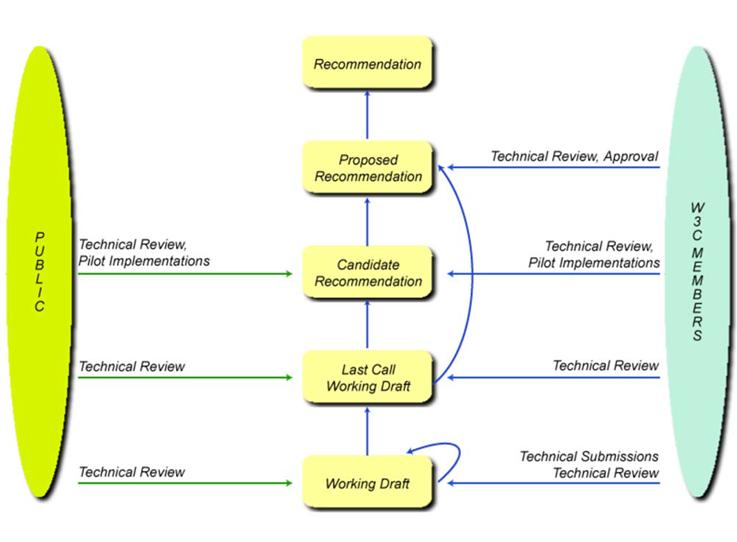
\includegraphics[width=\linewidth]{Images/W3C_Recommendation_Process.jpg}
        \caption{W3C recommendation process}
\end{figure}

The W3C uses a formal system of maturity levels to signal a technical report's status within the standardization process. These levels inform the community about the document's stability and the nature of the feedback being sought. \\

\textit{It is worth noting that the W3C standardization process differs from that of the IETF. While the latter publishes standards in the form of Requests for Comments (RFCs), the W3C adopts its own maturity levels, culminating in W3C Recommendations.}

\begin{itemize}
    \item 
    \textbf{Working Draft (WD):} A Working Draft is a document that the W3C has published for community review. It is considered a work in progress and is republished whenever significant changes are made, allowing stakeholders to track its evolution.

    \item 
    \textbf{Candidate Recommendation (CR):} A Candidate Recommendation is a document that the Working Group believes is technically complete and satisfies its requirements. At this stage, the group is seeking wide review and, crucially, implementation experience to validate the specification in practice.

    \item 
    \textbf{Proposed Recommendation (PR):} This is a mature technical report that has successfully passed technical reviews and has been formally submitted by the Director to the W3C membership for final endorsement. This stage signifies that the document is of sufficient quality to become a formal standard.

    \item 
    \textbf{W3C Recommendation (REC):} This is the final stage. A W3C Recommendation is a specification or set of guidelines that has received significant consensus from W3C Members and the Director. The W3C recommends the wide deployment of its Recommendations as official standards for the Web.

    \item 
    \textbf{Working Group/Interest Group Notes:} Separately, the W3C also publishes Notes. These documents are published by Working Groups or Interest Groups for informational purposes, such as to share ideas or document best practices. They are explicitly not intended to be formal standards.
\end{itemize}

Through its layered organizational structure and a rigorous, consensus-driven standardization process, the World Wide Web Consortium provides the essential governance needed to guide the Web's coherent evolution, ensuring it remains an open, interoperable, and universal platform for generations to come.

\end{document}